\newpage\section{Introduction} On dit que l'auteur américain Isaac Asimov aurait \'ecrit que \begin{quote}La phrase la plus int\'eressante à entendre [...] -- celle qui annonce le plus de découvertes -- n'est pas ``Eurêka!" mais plutôt "Comme c'est \'etrange ... ".\end{quote}
Les ob\-ser\-va\-tions anormales ne sont pas que des signes avant-coureurs de grandes découvertes scientifiques, cependant -- les ob\-ser\-va\-tions inattendues peuvent gâcher les analyses ou indiquer l'existence de problèmes liés à la saisie ou au traitement des données. \par Il devient ainsi impératif  d'établir des protocoles de détection des anomalies et d'identifier des stratégies pour faire face à de telles ob\-ser\-va\-tions.
\subsection{Notions fondamentales et survol}
Les \textbf{valeurs aberrantes} sont des ob\-ser\-va\-tions qui sont \textbf{atypiques} par rapport aux autres caract\'eristiques de l'unit\'e d'ob\-ser\-vation, ou par rapport aux valeurs correspondantes des autres unit\'es. Les valeurs aberrantes sont donc des ob\-ser\-va\-tions qui  \textbf{diff\`erent des autres cas} ou qui contredisent les  \textbf{dependances connues} au sujet des donn\'ees.\footnote{Une ob\-ser\-va\-tion peut \'etre aberrante selon n'importe laquelle des variables, ou encore en combinaison.}% (information in this section is taken partly from \cite{DP_OW,DP_A,DP_T,DP_CBK}).
\par Il se peut qu'une ob\-ser\-va\-tion soit aberrante dans un contexte particulier, mais pas dans un autre. Prenons, par exemple, un homme adulte de 180cm de taille. Un tel homme se retrouve dans le 86i\`eme centile par rapport \`a la population masculine canadienne \cite{DP_HPC}, ce qui n'est pas inhabituel; en Bolivie, cependant, le même homme se retrouve dans le 99,9i\`eme centile \cite{DP_HPC}, ce qui le marque comme un g\'eant par rapport \`a la population masculine bolivienne.\footnote{La détection d'anomalies devrait mener \`a se poser des questions suppl\'ementaires -- pourquoi y a-t-il un tel écart entre les deux populations?}
\newl
Les anlaystes commettent parfois une erreur fondamentale en retirant les valeurs aberrantes de l'ensemble de données sans d\'eterminer au pr\'ealable si ce sont des \textbf{ob\-ser\-va\-tions influentes}, c'est-à-dire des ob\-ser\-va\-tions dont l'absence entraîne des résultats d'analyse \textbf{nettement différents}.\par Lorsque de telles ob\-ser\-va\-tions sont identifiées, on doit d'abord appliquer des mesures correctives afin de minimiser tout effet ind\'esirable. Il est \`a noter que les valeurs aberrantes peuvent \^etre influentes, et que des ob\-ser\-va\-tions influentes peuvent être des valeurs aberrantes, mais les conditions ne sont ni nécessaires, ni suffisantes.
\subsubsection*{La d\'etection d'anomalies}  Par d\'efinition, les anomalies sont \textbf{peu fréquentes}, et typiquement enrob\'ees d'\textbf{incertitude} en raison de leur petit nombre relatif, ce qui complique leur  différenciation d'un simple \textbf{bruit} ou d'\textbf{erreurs de saisie de donn\'ees}. \par De plus, la fronti\`ere entre les unités normales et les unités déviantes est en g\'en\'eral \textbf{floue}; avec l'avènement des boutiques en ligne, par exemple, un achat enregistr\'e à 3h du matin ne sonne plus nécessairement l'alarme. \par Il est déjà assez difficile d'essayer d'identifier les anomalies "honnêtes"; lorsque elles sont en fait associées à des \textbf{activités malveillantes}, elles sont typiquement \textbf{déguisées} afin de ressembler à des ob\-ser\-va\-tions normales, ce qui peut venir compliquer les choses.  
\newl
Aucune des nombreuse m\'ethodes de d\'etection des ano\-malies n'est infaillible. Les méthodes qui utilisent des aides graphiques (comme les diagrammes de boîtes \`a moustache ou les nuages de points) pour identifier les valeurs aberrantes sont particulièrement faciles à mettre en oeuvre, mais l'interpr\'etation des graphiques demeurent compliqu\'ees en pr\'esence de donn\'es de haute dimension. \par Les méthodes analytiques (utilisant les distances de Cooke ou de Mahalanobis, par exemple) demandent en g\'en\'eral la conduite d'analyses supplémentaires, surtout lors de l'identification de donn\'ees influentes (\textit{cf.} ``\textbf{leverage}''). 
\newl Dans les petits ensembles de données, la détection d'ano\-ma\-lies peut être effectuée au cas par cas; avec des donn\'ees massives, les analystes doivent \'eviter la \textbf{détection/suppression automatisée} aveugle.\footnote{D\`es que les ob\-ser\-va\-tions "anormales" sont supprim\'ees de l'ensemble de données, les ob\-ser\-va\-tions qui \'etaient ant\'erieurement "régulières" peuvent à leur tour devenir anormales dans l'ensemble de données r\'eduit; quand le proc\'ed\'e est automatis\'e, il n'est pas \'evident qu'il s'arr\^etera avant qu'il ne reste  qu'une unique obvservation dans l'ensemble de donn\'ees.}\par
Aux premières \'etapes de la détection des anomalies, les analyses de donn\'ees \textbf{simples} (telles que le calcul de statistiques descriptives et de tableaux de contingence) peuvent aider  à identifier les ob\-ser\-va\-tions anormales ou \`a  obtenir un aperçu des données, ce qui peut éventuellement entra\^{\i}ner des modifications au plan d'analyse.
\subsubsection*{Tests de valeurs aberrantes} Les méthodes de d\'etection se situent dans l'un des deux camps: \textbf{supervis\'ee} et \textbf{non supervis\'ee}.
\par Les méthodes supervisées utilisent un historique d'ob\-ser\-va\-tions anormales (identifi\'ees au pr\'ealable par des sommit\'es en la mati\`ere) afin de construire un \textbf{mod\`ele pr\'edictif} qui estime la probabilité qu'une unité soit anormale. Les anomalies sont typiquement \textbf{peu fréquentes} et ces modèles doivent tenir compte du \textbf{problème des cas rares}.\footnote{Les modèles supervisés sont construits pour minimiser le co\^ut associ\'es aux erreurs d'identification; en g\'en\'eral, on suppose d'habitude que le coût des erreurs de classification est symétrique, ce qui peut conduire à des solutions techniquement correctes mais inutiles en pratique. Par exemple, la grande majorité (99,999+\%) des passagers aériens n'apportent pas d'articles interdits dans les avions; un modèle qui prédit qu'aucun passager ne tente d'introduire clandestinement une arme à bord d'un vol serait précis à 99,999+\%, mais il manquerait complètement le bateau.} \par Les méthodes non supervisées, quant \`a elles, n'utilisent pas d'information externe ("labels") afin de déterminer si une ob\-ser\-va\-tion est marginale; le verdict est rendu uniquement en comparant son comportement à celui des autres ob\-ser\-va\-tions.
\newpage\noindent Les m\'ethodes de d\'epistage des anomalies suivantes sont de cette cat\'egorie:\footnote{Pour la plupart de ces tests, on suppose que les valeurs \'etudi\'ees suivent une distribution \textbf{normale}; la robustesse des tests vis-\`a-vis un \'ecart par rapport `a cette hypoth\`ese s'\'etudie au cas par cas.}
\begin{itemize}[noitemsep]
\item le test le plus courrament utilis\'e est sans doute le  \textbf{test de la bo\^{\i}te \`a moustaches de Tukey}; si les valeurs sont distibu\'ees selon une normale, les \textbf{valeurs r\'e\-gu\-li\-\`eres} se retrouvent entre les \textbf{cl\^otures int\'erieures} $$Q_1-1.5(Q_3-Q_1) \quad\mbox{et}\quad Q_3+1.5(Q_3-Q_1).$$ Les \textbf{valeurs aberrantes suspect\'ees} se retrouvent entre ces derni\`eres et les \textbf{cl\^otures ext\'erieures} 
$$Q_1-3(Q_3-Q_1) \quad\mbox{et}\quad Q_3+3(Q_3-Q_1).$$
Les valeurs au-del\`a des clot\^ures ext\'erieures sont des \textbf{valeurs aberrantes} ($Q_1$ et $Q_3$ repr\'esentent respectivement le $1^{\textrm{er}}$ et le $3^{\textrm{e}}$ quartile des valeurs; consulter la figure~\ref{fig:boxplot}).
\begin{figure}[t]
\centering
\includegraphics[width=0.30\textwidth]{Images/boxplot_\ldoc.png}
\caption{\small Le test de la bo\^{\i}te \`a moustaches de Tukey; valeurs aberrantes (disques pleins), suspect\'ees (disques vides).}
\hrule\label{fig:boxplot}
\end{figure}
\afterpage{\FloatBarrier}
\item le \textbf{test de Grubbs} est un autre test univari\'e d'usage courant, prenant en consid\'eration le nombre d'ob\-ser\-va\-tions $N$. Soient  $(\overline{x},s_x)$ la moyenne et l'\'ecart-type de $X$; $\alpha$ le niveau de signification souhait\'e, et $T(\alpha,N)$ la valeur critique de la distribution $T$ de Student, pour une signification de $\alpha/2N$. La $i^{\textrm{e}}$ ob\-ser\-va\-tion est une \textbf{valeur aberrante selon} $X$ si $$|x_i-\overline{x}| \geq \frac{s_x(N-1)}{\sqrt{N}}\sqrt{\frac{T^2(\alpha,N)}{N-2+T^2(\alpha,N)}}.$$
\item on reconna\^{\i}t aussi les test suivants:
\begin{itemize}[noitemsep]
\item le \textbf{test $Q$ de Dixon}, qui est parfois utilisé afin de trouver des valeurs aberrantes dans de (tr\`es) petits ensembles -- sa validit\'e est douteuse;
\item la \textbf{distance de Mahalanobis}, qui est liée au "leverage" d'une ob\-ser\-va\-tion (une mesure de son influence), peut aussi être utilisés afin d'identifier des valeurs aberrantes selon plusieurs dimensions lorsque toutes les relations sont linéaires (ou presque);
\item le \textbf{test de Tietjen-Moore}, qui est utlis\'e afin de d\'eterminer un nombre sp\'ecifique d'anomalies;
\item le \textbf{test "ESD"} (une g\'en\'eralisation de Grubbs), quand le nombre d'anomalies est inconnu;
\item le \textbf{test du $\chi^2$}, lorsque les anomalies ont un effet sur la qualit\'e de l'ajustement, et,   
\item DBSCAN et les autres algorithmes de d\'etection qui se basent sur le "\textbf{clustering}". 
\end{itemize}
\end{itemize}
\subsubsection*{D\'etection visuelle} Les exemples simples qui suivent illustrent les principes qui sous-tendent la détection visuelle des valeurs aberrantes. 
\begin{Exemple} On mesure la taille de plusieurs plantes dans une pépinière. Les registres indiquent également l'âge de chaque plante (le nombre de semaines depuis que la semence a été plantée). 
\begin{figure*}[t]
\centering
\includegraphics[width=0.32\textwidth]{Images/plant_age_\ldoc}\quad
\includegraphics[width=0.32\textwidth]{Images/plant_height_\ldoc}\quad
\includegraphics[width=0.32\textwidth]{Images/plant_height_vs_age_\ldoc}
\caption{\small R\'esum\'e visuel d'un ensemble de donn\'ees artificiel: distibutions de l'\^age (\`a gauche) et de la taille des plantes (au centre), tendance lin\'eaire (\`a droite).} \label{fig:plant_data}
\end{figure*}
\begin{figure*}[t]
\centering
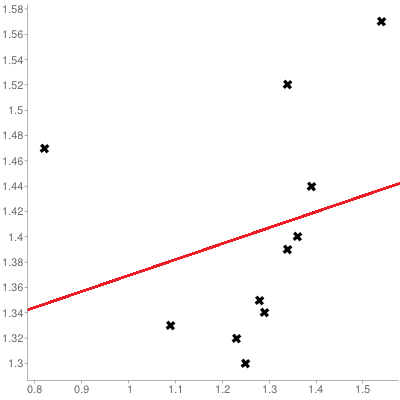
\includegraphics[width=0.32\textwidth]{Images/scatter_plot_linear_1}\quad
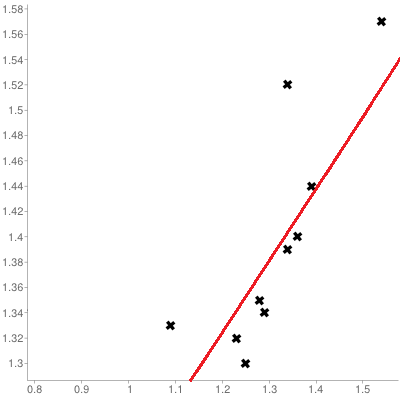
\includegraphics[width=0.32\textwidth]{Images/scatter_plot_linear_2}\quad
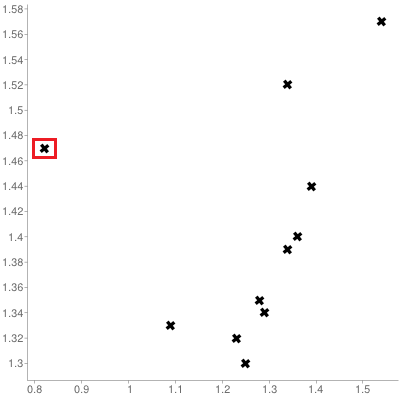
\includegraphics[width=0.32\textwidth]{Images/scatter_plot_2}
\caption{\small Visualisations des taux de services et d'achalandage: tendances lin\'eaire pour 11 bureaux (\`a gauche) et 10 bureaux (au centre), ob\-ser\-va\-tions influentes (\`a droite).}\hrule
        \label{fig:service_data}
\end{figure*}
\begin{figure*}[t]
\centering\includegraphics[width=0.26\textwidth]{{Images/appendage_length_descriptive_\ldoc}}\quad \includegraphics[width=0.55\textwidth]{{Images/appendage_length_\ldoc}}
\caption{\small R\'esum\'e et visualisation de la longeur des antennes: statistiques descriptives (\`a gauche), distribution (\`a droite).}\hrule
\label{tab:appendage_data}
\end{figure*}

Les histogrammes de l'\^age (\`a gauche) et de la taille (au centre) des plantes se retrouvent \`a la   figure~\ref{fig:plant_data}. Il n'y a que tr\`es peu \`a dire au sujet de ces distribution univari\'ees: l'\^age  (qui est control\'e par le peronnel de la p\'epini\`ere) semble désordonné, tout comme l'est la variable réponse (taille). Un nuage de points (figure~\ref{fig:plant_data}, \`a droite), cependant, révèle que la croissance est fortement corrélée avec l'âge pendant les premiers instants de la vie d'une plante; les points se regroupent autour d'une tendance linéaire. Un point en particulier (en jaune) est ais\'ement  identifiable comme \textbf{valeur aberrante}.\par Il y a (au moins) deux possibilités: soit l'\^age ou la taille de cette plante a mal \'et\'e saisie, soit un spécimen a connu une croissance inhabituelle. Quoi qu'il en soit, l'analyste doit enquêter davantage.  
  \end{Exemple}
  \begin{Exemple}
Un ministère poss\`ede 11 bureaux de service sur son territoire. Les statistiques de service sont enregistrées: les taux moyens mensuels d'arrivée et de service par guichet pour chaque point de service sont disponibles. \par Un  diagramme de dispersion des taux de service (axe des $y$) par rapport au taux d'arrivée  (axe des $x$), avec tendance  linéaire, est présenté \`a la figure~\ref{fig:service_data} (\`a gauche). La tendance est à la hausse lorsque les valeurs de $x$ augmentent. Un diagramme similaire est pr\'esent\'e \`a la figure~\ref{fig:service_data} (au centre), mais avec le point le plus à gauche retiré de l'ensemble de donn\'ees. La tendance est toujours à la hausse, mais l'ajustement est significativement amélioré, ce qui suggère que l'ob\-ser\-va\-tion supprimée est indûment \textbf{influente} (ou anormale) -- on obtient une meilleure compréhension de la relation entre les arrivées et les services si elle est mise de côté. Toute tentative d'intégration de cette observation dans le modèle doit  en tenir compte. On note, cependant, que les observations influentes dépendent de l'analyse qui est menée en bout du compte -- un point peut avoir de l'influence dans une analyse, mais pas dans une autre.   
\end{Exemple}
\begin{Exemple}
On a mesur\'e la longeur des antennes de 71 sp\'ecimens d'une esp\`ece d'insecte; les statistiques descriptives de l'\'echantillon sont pr\'esent\'ees \`a la figure~\ref{tab:appendage_data} (\`a gauche).
\newpage\noindent Les analystes bien inform\'es reconnaîtront les signes révélateurs que la distribution des longueurs d'antennes est susceptible d'être asymétrique (puisque l'asymétrie n'est pas négligeable) et d'avoir une queue ``grasse'' (le kurtosis étant proportionnel à la moyenne et à l'écart type, l'étendue étant beaucoup plus grande que l'\'ecart interquartile, et le maximum étant beaucoup plus \'elev\'e que le 3e quartile). \par Les valeurs du mode, du minimum, et du premier quartile sont associ\'ees à des sp\'ecimens sans antennes -- il semble y avoir au moins deux sous-groupes dans la population (peut-être répartis en catégories jeunes/adultes, ou femelles/m\^ales). La valeur maximale, ayant déjà été not\'ee comme étant \'elev\'ee par rapport \`a la plupart des ob\-ser\-va\-tions, est une valeur aberrante en potentiel. \par L'histogramme des mesures montre cependant qu'il y a 3 sp\'ecimens dont les antennes sont très longues, comme on peut le constater \`a la figure~\ref{tab:appendage_data} (\`a droite): il devient maintenant plausible que ces entrées anormales appartiennent à des sp\'ecimens d'une espèce différente qui ont été ajout\'e par erreur aux donn\'ees recueillies. Cela ne constitue pas, bien sûr, une preuve sans \'equivoque  d'une telle erreur, mais cela en soulève la possibilité, ce qui est souvent la mieux que l'analyste puisse faire en absence d'expertise en la matière.
\end{Exemple}
\noindent Cependant, l'approche traditionnelle ne fonctionne pas en g\'en\'eral pour les ensembles de grande dimension et une approche fondamentalement différente est préconisée.\newpage  
\subsection{D\'etection d'anomalies et apprentissage automatique}
Les comportements frauduleux ne sont pas toujours facile \`a  identifier, même avec le recul. Les fraudeurs de cartes de crédit, par exemple, tentent de déguiser leurs efforts avec des transactions banales et r\'eguli\`eres, plutôt qu'ex\-tra\-va\-gantes, afin de tromper les observateurs humains et les amener à confondre ce qui est simplement \textbf{plausible} avec ce qui est \textbf{probable} (ou, tout du moins, \textbf{pas improbable}).\par À un niveau élémentaire, la détection d'anomalies est un problème de \textbf{probabilit\'e appliqu\'ee}: si $I$ indique ce que l'on sait au sujet des données (comportement individuel des ob\-ser\-va\-tions, comportement collectif, verdict r\'eguli\`ere/anormal pour plusieurs ob\-ser\-va-tions , etc.), est-ce que  $$P(\text{obs.\@ anormale}|I) > P(\text{obs.\@ normale}|I)?$$ 
Les modèles de détection des anomalies assument en g\'en\'eral la  \textbf{stationnarité des ob\-ser\-va\-tions normales}, c'est-à-dire que le mécanisme sous-jacent qui engendrent les données ne change pas de manière substantielle dans le temps, ou qu'il change avec un taux ou un caractère cyclique connu. \par Pour les données de séries chronologiques, il faut d'abord effectuer l'extraction de la tendance et de la saisonnalité.
\begin{Exemple} Les chaînes d'ap\-pro\-vi\-sion\-ne\-ment jouent un rôle crucial dans le transport des marchandises. Comme le  dit le proverbe, "une chaîne n'est pas plus solide que son maillon le plus faible" -- dans un contexte multimodal, il n'est pas \'evident de comparer les différents segments de transport: si les expéditions partant de Shanghai en février 2013 ont mis en moyenne deux jours de plus pour arriver à Vancouver que celles partant en juillet 2017, peut-on affirmer avec certitude que le proc\'ed\'e de transport s'est amélioré au fil des ans? ? \par La variabilité saisonnière de la performance est une mesure pertinente lors du monitorage des chaînes d'ap\-pro\-vi\-sion\-ne\-ment, et la capacité de quantifier son impact sur les données saisies est donc d'un grand intérêt. \par 
On peut aborder le probl\`eme \`a l'aide d'un \textbf{indice} de temps de transit pour les conteneurs. Cet indice devrait représenter la \textbf{fiabilit\'e} et la \textbf{variabilit\'e} des temps de transit, mais de manière à permettre la comparaison des performances d'une p\'eriode \`a une autre.
\newl On simplifie la discussion en prenant pour acquis que l'ob\-jec\-tif est de comparer les données de performance trimestrielles et/ou mensuelles, quelle que soit la saison de transit, afin de déterminer la performance du réseau dans le corridor \textit{Shanghai} $\to$ \textit{Port Metro Vancouver/Prince Rupert} $\to$ \textit{Toronto}, par exemple. 
\begin{figure}[H]
\centering
\includegraphics[width=0.48\textwidth]{Images/mmsc_\ldoc.png}
\caption{\small Chaînes d'ap\-pro\-vi\-sion\-ne\-ment multimodale.} \label{fig:mmsc}
\end{figure}
\noindent Les conteneurs quittent Shanghai par bateau, entrent au Canada et s\'ejournent dans le ports de Vancouver ou de Prince Rupert, pour ensuite continuer leur chemin par tain jusqu'\`a Toronto. \par 
Pour chacun des trois segments (transit maritime, s\'ejour portuaire, transit ferroviaire), les données sont form\'ees par la distribution empirique mensuelle des temps de transit, construite à partir d'échantillons repr\'esentatifs (sélectionnés au hasard) de tous les conteneurs entrant dans le segment approprié.
\newl
La performance de chaque segment est mesurée gr\^ace a divers \textbf{indicateurs de fluidit\'e} qui sont calculés à l'aide de  statistiques sur la distribution des temps de transit et de séjour pour chacun des segments de la chaîne: 
\begin{description}[noitemsep]
\item[indicateur de fiabilit\'e (RI)] -- le rapport du 95$^{\text{e}}$ centile au 5$^{\text{e}}$ centile de la distribution des temps de transit ou de s\'ejour (une valeur \'elev\'ee indiquant une forte volatilit\'e, tandis qu'une faible valeur RI $(\approx 1)$ indique un corridor fiable);
\item[indice tampon (BI)] -- le rapport de la diff\'erence positive entre le 95$^{\text{th}}$ centile et la moyenne, \`a la moyenne. Une faible valeur BI $(\approx 0)$ indique une l\'eg\`ere  variabilit\'e dans le r\'egime des longs temps de transit/s\'ejour, tandis qu'une valeur de BI \'elev\'ee indique une forte variabilit\'e  et la pr\'esence \'eventuelle de valeurs aberrantes dans ce m\^eme r\'egime;
\item[coefficient de variation (CV)] -- le rapport de l'\'ecart type \`a la moyenne des temps de transit/s\'ejour.  
\end{description}
Les séries chronologiques d'indicateurs mensuels (dérivées \`a partir des distributions mensuelles du temps de transit/s\'ejour dans chaque segment) sont alors \textbf{decomposées}:
\begin{itemize}[noitemsep]
\item composante de tendance;
\item composante saisonnière (saisonnalité, jour ouvrable, jour férié mobile), et 
\item composante irrégulière.
\end{itemize}
\noindent La composantes de tendance et la composante saisonnières forment le \textbf{comportement attendu} de la série chro\-no\-lo\-gi\-que des indicateurs;\footnote{Avant de procéder à la désaisonnalisation, il est important d'identifier et de pré-ajuster les ruptures structurelles (en utilisant le test de Chow, par exemple) car leur présence peut donner lieu à de graves distorsions dans l'estimation des effets de tendance et de saisonnalit\'e. Lorsque le niveau d'activité saisonnier habituel change, on a affaire \`a une rupture saisonni\`ere; les ruptures de tendance se produisent lorsque la tendance d'une série de données est réduite ou augmentée pendant une période prolongée, de façon temporaire ou permanente. Ces ruptures peuvent provenir de modifications aux politiques gouvernementales, de grèves, d'événements exceptionnels, d'intempéries, etc.} on doit la composante irrégulière \`a la \textbf{volatilit\'e} de la chaîne d'approvisionnement. Une composante irrégulière élevée (à un moment donné) indique une mauvaise performance par rapport aux attentes pour ce mois, c'est-à-dire que c'est une \textbf{valeur aberrante}.  
\begin{figure}[t]
\centering
\includegraphics[width=0.5\textwidth]{Images/decomposition_\ldoc.png}
\caption{\small Décomposition conceptuelle d'une série chronologique; c'est dans la composante irrégulière qu'il faut chercher les valeurs aberrantes.}\hrule \label{fig:description}
\end{figure}
\newl En g\'en\'eral, la decomposition s'effectue selon un mod\`ele 
\begin{itemize}[noitemsep]
\item multiplicatif;
\item additif, ou encore 
\item pseudo-additif.
\end{itemize}
Le choix de modèle dépend du comportement des données et de la s\'election des hypothèses; X12 permet d'automatiser certains aspects de la décomposition, mais une intervention manuelle lors de la phase du diagnostique demeure essentielle.\footnote{X12 est implémenté dans SAS et R, entre autres plateformes.}
Le modèle additif, par exemple, suppose que: 
\begin{enumerate}[noitemsep]
\item les composantes saisonni\`ere $S_t$ et irr\'eguli\`eres $I_t$ sont ind\'ependentes de la tendance  $T_t$; 
\item la composante saisonni\`ere $S_t$ demeure stable d'une ann\'ee \`a l'autre, et 
\item la fluctuation saisonni\`ere totale est $\sum_{j=1}^{12} S_{t+j}=0 $.\end{enumerate} 
Mathématiquement, le modèle s'exprime sous la forme
    \begin{equation*}
        O_t = T_t + S_t + I_t
    \end{equation*}
    Les composantes partagent toutes les mêmes dimensions. La série désaisonnalisée prend la forme
    \begin{equation*}
        SA_t = O_t - S_t = T_t + I_t
    \end{equation*}
Les modèles multiplicatif et pseudo-additif sont définis de la même manière (consulter  \cite{TS_FH,TS_FMBOC,TS_ICTSA,TS_SAETS,TS_JL} pour plus de détails).\footnote{Si l'ampleur de la variation saisonnière augmente (ou diminue) avec le temps, la décomposition multiplicative est de mise. Par contre, si la variation saisonnière constante dans le temps, on pr\'econise un modèle additif. Lorsque les donn\'es pr\'sentent les caract\'eristiques du mod\`ele multiplicatif mais que les valeurs des paramètres associ\'es se rapprochent de zéro, on a affaire au mod\`ele pseudo-additif.}\newl 
Le proc\'ed\'e de décomposition et de préparation des données est illustré \`a l'aide d'une série chronologique  pour le CV mensuel du transit maritime, de 2010 à 2013 (40 mois), dont les valeurs se retrouvent à la figure~\ref{fig:cv_cont}. La taille des pics et des creux semble relativement constante par rapport à la tendance en \'evolution; l'implémentation SAS de X12  est en accord avec cette évaluation et suggère une décomposition additive (sans qu'il soit nécessaire de transformer davantage les données).
\begin{figure*}[t]
\centering
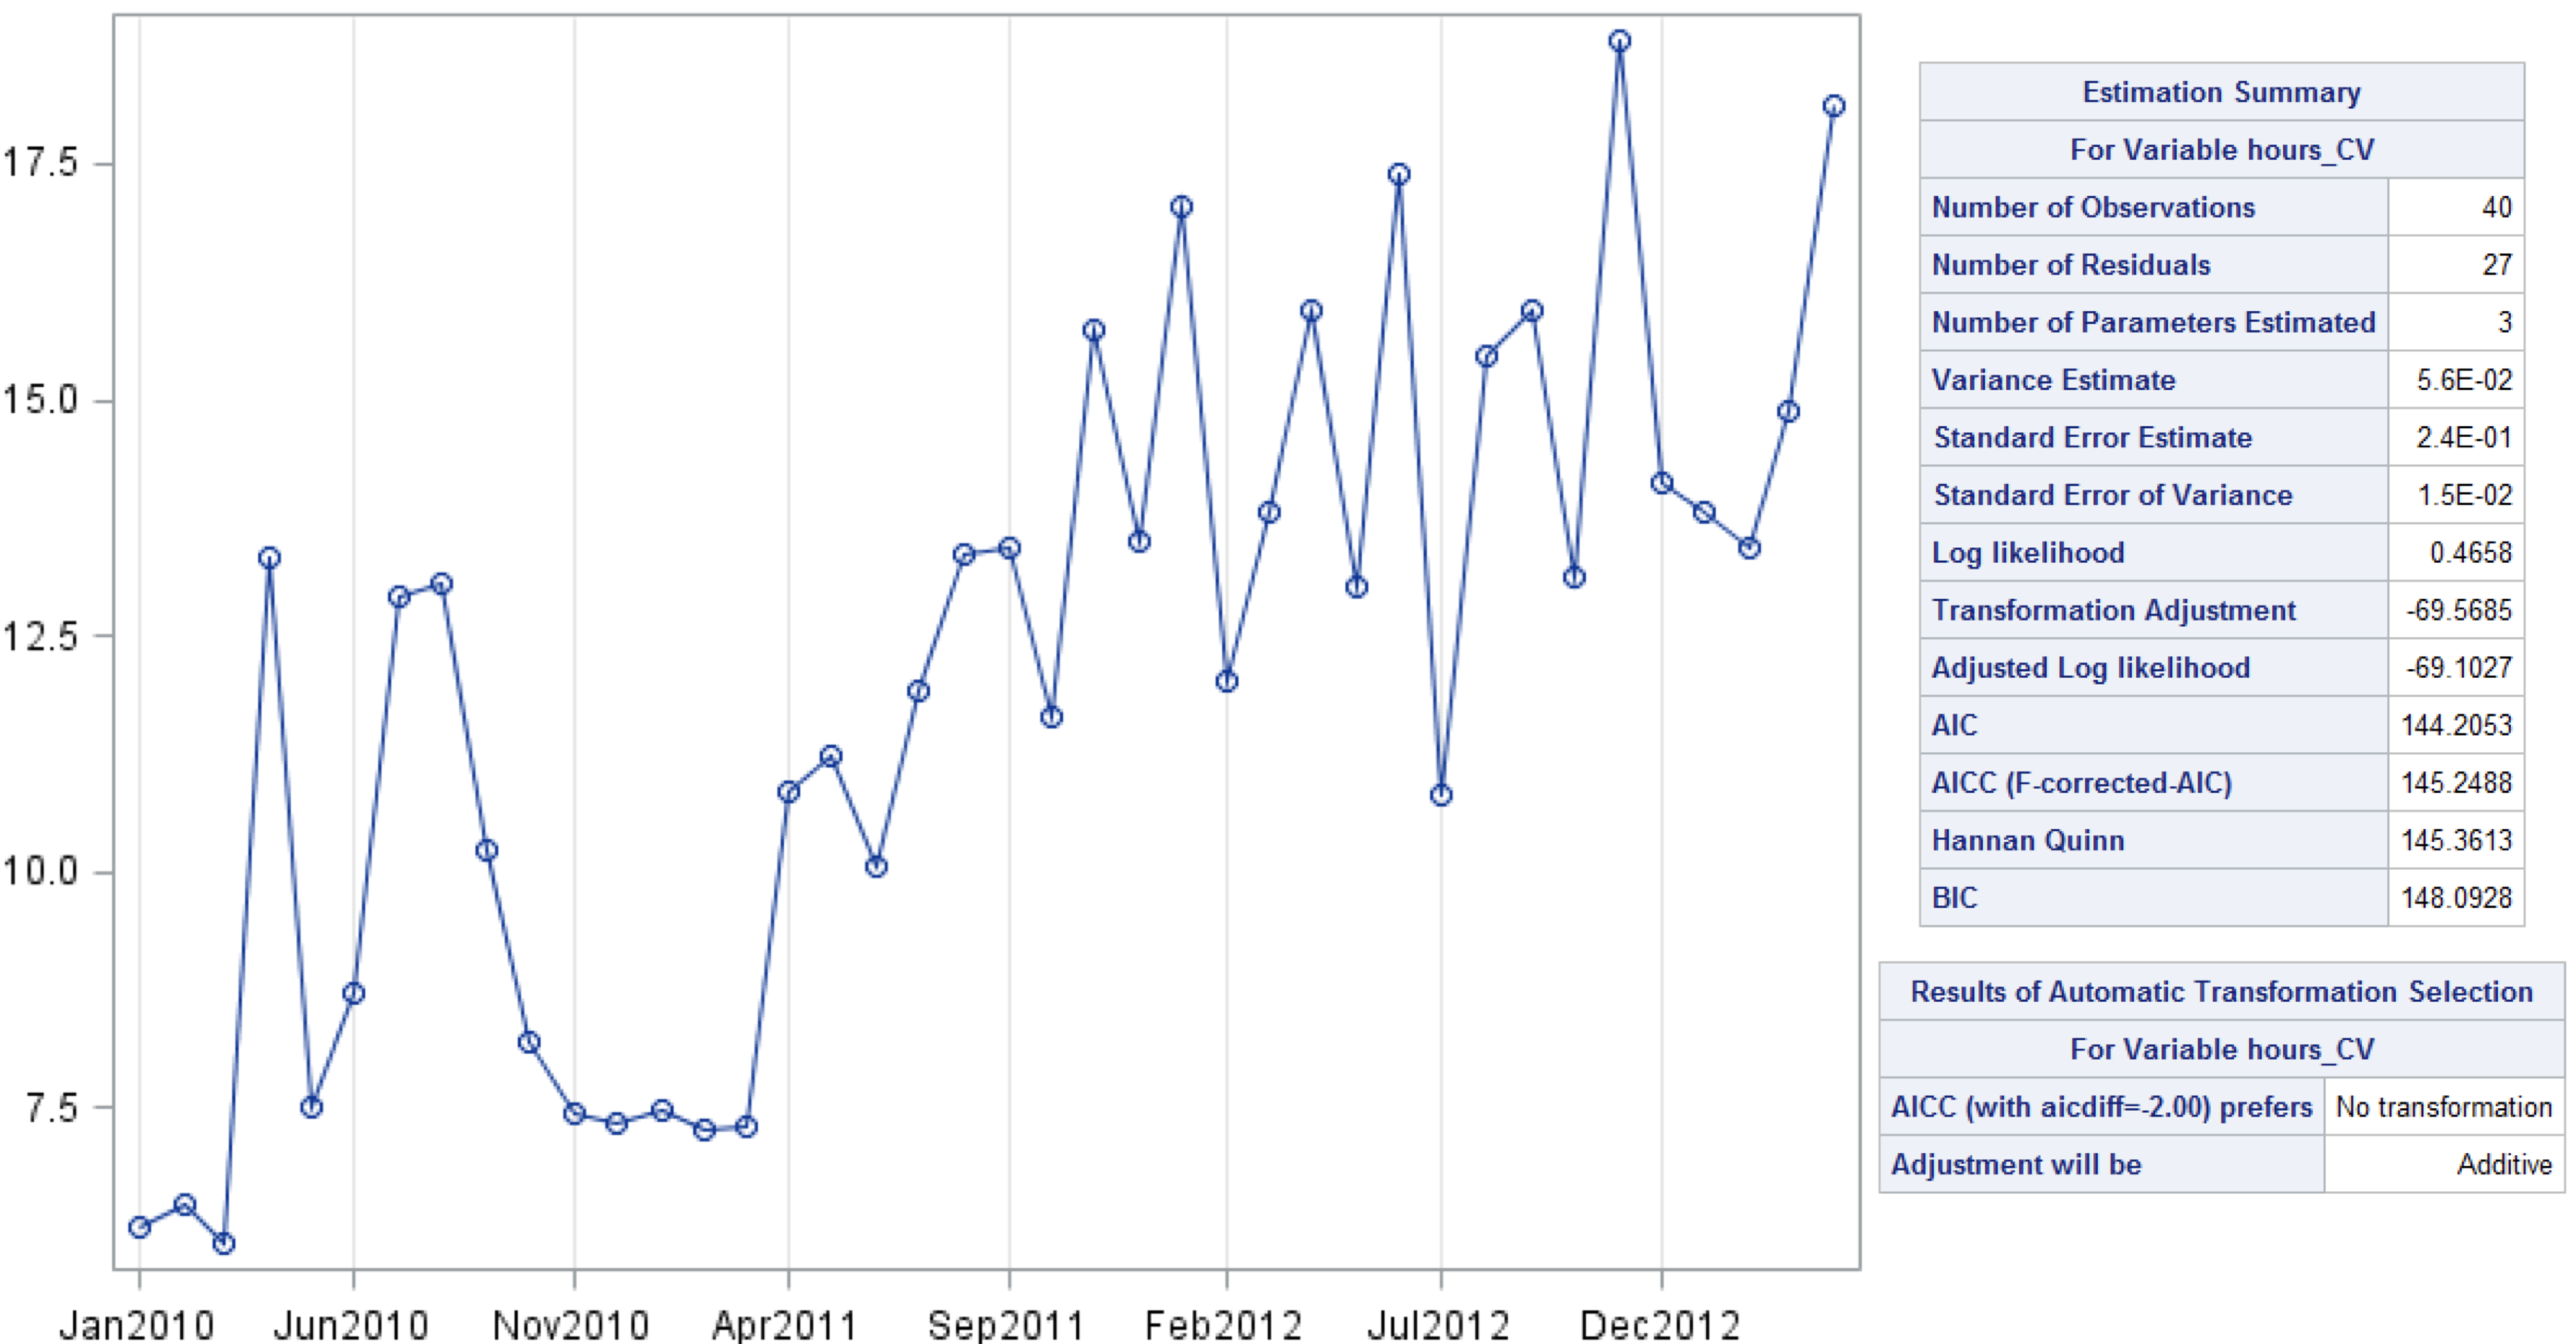
\includegraphics[width=0.75\textwidth]{Images/CV_continuously.png}
\caption{\small CV mensuels du transit maritime Shanghai $\to$ Vancouver/Prince Rupert; r\'esum\'e d'estimation.}
\label{fig:cv_cont}
\end{figure*}
\par Les courbes de diagnostique sont présentées \`a la figure~\ref{fig:diff}: la série des CV est préajustée de JAN2010 à OCT2010 en raison d'un décalage de niveau d\'etect\'e. Le graphique SI ("seasonal irregular chart") montre que la composante irr\'eguli\`ere comprend une certaine volatilit\'e (JUN2010, JUL2010, etc.)
\begin{figure*}[t]
\centering
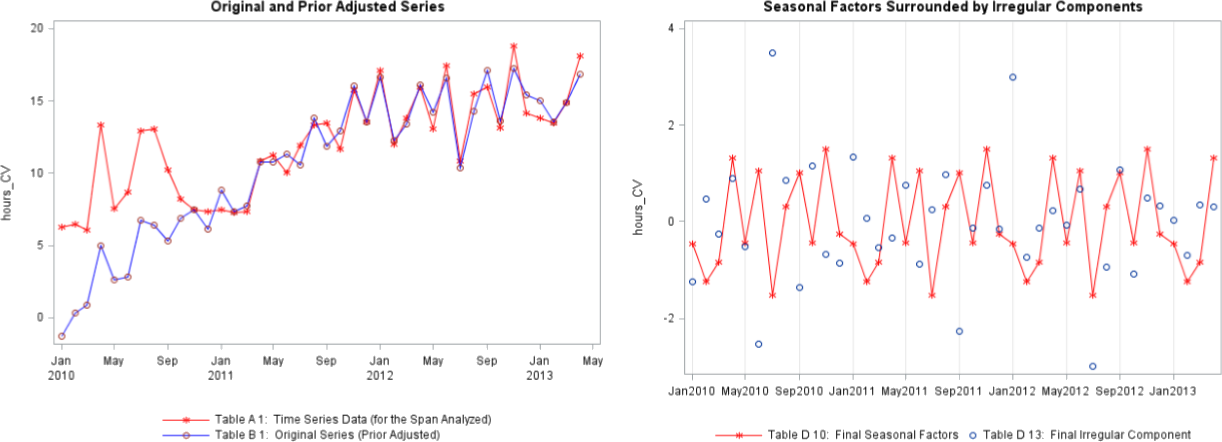
\includegraphics[width=0.98\textwidth]{Images/DiffComponents.png}
\caption{\small Graphiques de diagnostique. On note que l'analyse d'une série chronologique commence par l'estimation des effets de jours f\'eri\'es mobiles et des jours ouvrables, qui sont ensuite utilisés lors du rajustement préalable de la série. La série originale ajustée antérieure est ensuite analysée à l'aide de la désaisonnalisation.}\hrule
\label{fig:diff}
\end{figure*}
On montre la série ajustée \`a la figure~\ref{fig:adjusted}; les composantes de tendance et irrégulière sont également pr\'esent\'ees séparément afin d'offrir une meilleure lisibilité. C'est dans la composante irréguli\`ere que l'on cherche les anomalies. 
\begin{figure*}[t]
\centering
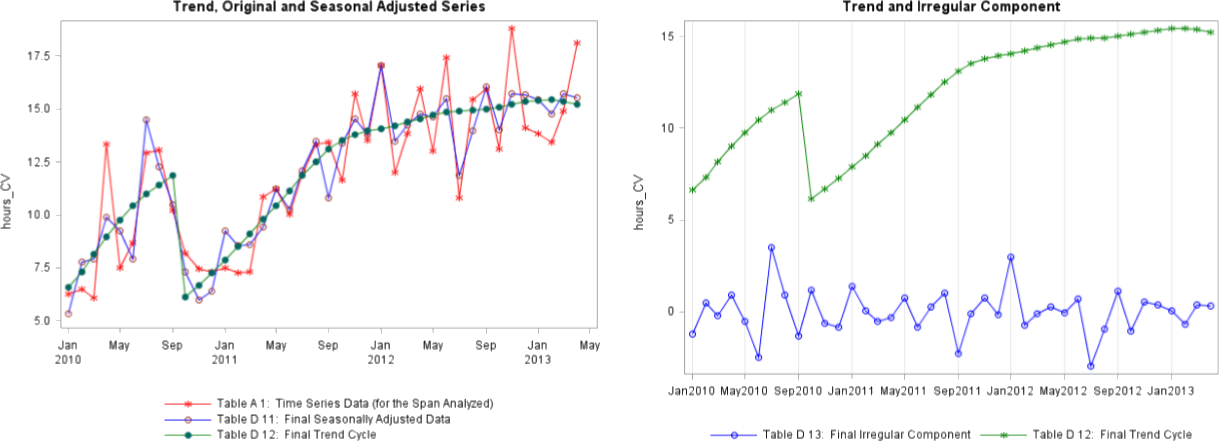
\includegraphics[width=0.98\textwidth]{Images/adjustedplot.png}
\caption{\small Diagrammes des composantes de la série chronologique ajustée.}\hrule
\label{fig:adjusted}
\end{figure*}
\end{Exemple}
\begin{center}
    \rule{0.25\textwidth}{.4pt}
\end{center}
Il existe d'autres approches conceptuelles: on peut considérer l'indentification des valeurs aberrantes comme un problème de \textbf{classification de cas rares} ou encore comme un problème de \textbf{d\'etection de nouveaut\'es} dans un  flux de données (ces problèmes seront traités dans les autres rapports de cette série sur la science des donn\'ees). \par D'une façon ou d'une autre, bien qu'un certain nombre de stratégies utilisent des algorithmes de classification ou de "clustering", elles sont rarement efficaces à moins de n'\^etre adaptées ou modifiées pour le contexte sp\'ecifique de la détection des anomalies.  
\subsubsection*{Notions fondamentales}
Un système générique (tel que celui des temps de transit/s\'ejour mensuels de la sous-section précédente, par exemple) peut être réalisé dans des états \textbf{normaux} ou \textbf{anormaux}. Cependant, la normalité, peut-être de mani\`ere contre-intuitive, ne se limite pas à trouver l'état le plus probable car des états peu fréquents pourraient être tout du moins normaux (ou plausibles) selon certaines interprétations du système. \par Selon \cite{A10}, les états d'un système sont le résultat de proc\'ed\'es ou de comportements qui suivent certaines règles naturelles et principes généraux; les ob\-ser\-va\-tions de l'ensemble de donn\'ees sont une manifestation de ces états. En général, les données permettent de tirer des conclusions sur les proc\'ed\'e sous-jacents, qui peuvent ensuite être testées ou invalidées par une saisie de données supplémentaires. Lorsque le syst\`eme est perturbées, ses \'etats risquent également de l'être perturbées; si une anomalie survient à la suite d'un proc\'ed\'e perturbé, la d\'etection des anomalies revient \`a identifier quand c'est le proc\'ed\'e qui est anormal. 
\newl Tout algorithme \textbf{supervisé} de détection d'anomalies n\'ecessite un ensemble de données historiques étiquetées (ce qui peut être tr\`es coûteux à obtenir) sur lequel on construit le modèle de prédiction, et un ensemble de validation sur lequel évaluer la performance du modèle en termes de \textbf{vrais positifs} ($\text{VP}$, anomalies d\'etect\'ees résultant  de procédés anormaux); \textbf{vrais n\'egatifs} ($\text{VN}$, ob\-ser\-va\-va\-tions normales prédites qui découlent  de procédés normaux); \textbf{faux positifs} ($\text{FP}$, anomalies détectées correspondant à des proc\'ed\'es réguliers), et \textbf{faux négatifs} ($\text{FN}$, ob\-ser\-va\-tions normales prédites qui sont en fait le produit de proc\'ed\'es anormaux). \newpage\noindent
\qquad\includegraphics[width=0.4\textwidth]{Images/Confusion_\ldoc.png}\par\noindent
Le contexte des cas rares fait en sorte que la meilleure strat\'egie ne consiste pas \`a maximiser le nombre de bonnes pr\'edictions ("\textbf{accuracy}"\footnote{Le terme n'est pas traduit, en g\'en\'eral.}) $$a=\frac{\text{VN}+\text{VP}}{\text{VN}+\text{VP}+\text{FN}+\text{FP}};$$ il faut au contraire essaayer de minimiser les taux d'erreur FP et FN, en gardant en t\^ete que le co\^ut associ\'e \`a un FN pourrait \^etre beaucoup plus \'elev\'e que celui associ\'e \`a un FP. \newpage \noindent Si un ensemble de validation contient $d=\text{FN}+\text{VP}$ anomalies r\'eelless, et qu'un algorithme de détection identifie $m=\text{FP}+\text{VP}$ ob\-ser\-va\-tions suspectes, dont $n=\text{VP}$ sont en fait des valeurs aberrantes, la performance de l'algorithme est souvent mesurée à l'aide de: 
\begin{description}
\item[pr\'ecision]-- la proportion de valeurs aberrantes r\'eeles parmi les observations suspectes $$p=\frac{n}{m}=\frac{\text{VP}}{\text{FP}+\text{VP}};$$ lorsque la plupart des points identifiés par l'algorithme sont en fait des valeurs aberrantes, $p\approx 1$ ;
\item[rappel]-- la proportion des valeurs aberrantes correctement identifi\'ees par l'algorithme
$$r=\frac{n}{d}=\frac{\text{VP}}{\text{FN}+\text{VP}};$$ lorsque la plupart des valeurs aberrantes sont identifi\'ees par l'algorithme, $r\approx 1$;
\item[mesure $F_1$]-- la moyenne harmonique de $p$ et $r$ 
$$F_1=\frac{2pr}{p+r}=\frac{2\text{VP}}{2\text{VP}+\text{FP}+\text{FN}};$$ ni la précision, le rappel, ou la mesure $F_1$ n'utilisent les $\text{VN}$ lors de l'évaluation, ce qui est un inconv\'enient.\footnote{L'analyste pour qui la vision globale est importante devrait aussi évaluer l'algorithme à l'aide du \textbf{coefficient de corrélation de Matthews} \cite{W_MCC} ou de la \textbf{sp\'ecificit\'e} $s=\frac{\text{VN}}{\text{FP}+\text{VN}}$.}
\end{description}
\begin{Exemple}Soit un ensemble de validation avec 5000 ob\-ser\-va\-tions, dont 100 sont anormales. Un algorithme pour lequel toutes les ob\-ser\-va\-tions sont anormales obtiendrait $a=p=0.02$, $r=1$, et $F_1\approx 0.04$, tandis qu'un algorithme qui détecte 10 des valeurs extrêmes réelles obtiendrait $r=0.1$ (les autres statistiques d\'ependent de $\text{VN}$ et $\text{FN}$).
\end{Exemple}
\newpage \noindent On peut aussi essayer d'estimer "l'anormalit\'e  relative" de diverses ob\-ser\-va\-tions: quoiqu'il est en g\'en\'eral assez difficile d'estimer directement la probabilité qu'une ob\-ser\-va\-tion $\mathbf{x}_1$ soit anormale, on peut parfois d\'eterminer qu'elle est plus probable de l'\^etre qu'une autre ob\-ser\-va\-tion $\mathbf{x}_2$ ($\mathbf{x}_1\succeq \mathbf{x}_2$). %\par Either way, it is usually preferable to attempt to estimate $P(\mathbf{x}\text{ is an anomaly}|I)$ rather than to attempt to predict $\text{class}(\mathbf{x})\in\{\text{anomaly},\text{normal}\}$ directly. 
\par Ce paradigme permet de classer les ob\-ser\-va\-tions suspectes; soit $k_i\in\{1,\ldots,m\}$ soit le rang de la $i^{\text{th}}$ valeur aberrante r\'eelle dans la liste des ob-ser\-tions suspectes, $i\in \{1,\ldots,n\}$, c'est-\`a-dire que $$\mathbf{x}_1\succeq \mathbf{x}_{k_1}\succeq \cdots\succeq\mathbf{x}_{k_i}\succeq \cdots \mathbf{x}_{k_n}\succeq \mathbf{x}_m;$$ le "\textbf{rank power}" de l'algorithme est donn\'e par $$RP=\frac{n(n+1)}{2\sum_{i=1}^nk_i}.$$ Lorsque les $d$ anomalies réelles se retrouvent dans les $d$ premières ob\-ser\-va\-tions suspectes, $RP= 1$. Le ``rank power'' n'est bien défini que lorsque $m\geq d$. \par Il faut \'eviter d'\'evaluer la performance d'un unique algorithme; c'est en comparaison avec la performance des autres algorithmes que les m\'etriques s'av\`erent \^etre utiles.  \newl Du côté des m\'ethodes \textbf{non supervis\'ees}, on consid\`ere que les anomalies sont des ob\-ser\-va\-tions qui sont différentes des autres. Si les ``clusters'' représentent des regroupements d'ob\-ser\-va\-tions semblables, celles qui n'appartiennent pas naturellement \`a un ``cluster'' sont des anomalies potentielles (consulter la figure~\ref{fig:clust2}). \par Il y a plusieurs d\'efis \`a relever; dont le choix  d'une mesure de similarité ou de dissimilarité des observations n'est pas le moindre (différentes mesures pouvant mener à différentes assignations des ``clusters''). \newl Enfin, il convient de mentionner que les définitions de termes comme \textbf{normales} et \textbf{anormales} sont laiss\'es volontairement vagues, afin d'offrir une  une certaine flexibilité aux analystes. 
\begin{figure*}[t]
\centering
\includegraphics[width=\textwidth]{Images/clustering2_\ldoc.png}
\caption{\small Regroupement de clients (rouge, vert, bleu) et valeurs aberrantes en potentiel (gris) dans un ensemble artificiel.}\hrule\label{fig:clust2}
\end{figure*}

\subsection{Sources importantes}
\newpage
\subsection{Structure et organisation du rapport}
Dans ce rapport, nous visons à fournir une meilleure compréhension de la détection des anomalies, des techniques de détection des valeurs aberrantes ainsi que des défis connexes associés. 

L'objectif de la section \ref{Section:2} est de fournir un aperçu complet et structuré des différentes méthodes de détection des anomalies et d'analyse des valeurs aberrantes dans le \textbf{cas quantitatif}, tandis que le \textbf{cas qualitatif} est abordé \`a la section \ref{Section:3}. Dans ces sections, une attention particulière sera accordée aux méthodes \textbf{supervisées} et aux méthodes \textbf{non-supervisées}, en autres avec les méthodes \`a base de la \textbf{distance} et de la \textbf{densité}. La section \ref{Section:4} est consacrée aux approches pour les \textbf{grands ensembles de données}, connues sous le nom de HDLSS (``\textbf{high dimension low sample size}'') où la taille de l'échantillon $n$ est inférieure à la dimension $p$. La détection des valeurs aberrantes dans les ensembles de données HDLSS est encore plus difficile en raison principalement du \textbf{fléau de la dimensionnalité}. La méthode des \textbf{ensembles et sous-espaces} anisi que certaines méthodes de réduction de la dimension y sont étudiées. Enfin, dans les sections \ref{Section:5} et \ref{Section:6}, des exemples pratiques seront étudiés en détail avec des données réelles provenant de plusieurs contextes.
\newpage